In the last section, frequency distribution tables were used to summarize the model validation results of a single constraint and it is shown how multiple grouping functions can be merged together. Here these concepts are used to decompose the confusion matrix w.r.t to the constraint validation results. 

The confusion matrix is a tool often used when evaluating a machine learning model $M_\theta$ trained on a classification task and is basically a frequency distribution table \cite{fawcett2006introduction}. Given a classification task, the confusion matrix counts the number of samples $(\mathbf{x}_i, t_i) \in D$ with $M_\theta(\mathbf{x}_i) = t_i$ (true positives), $M_\theta(\mathbf{x}_i) \neq t_i$ (false positives), $M_\theta(\mathbf{x}_i) = t_i$ (true negatives), and $M_\theta(\mathbf{x}_i) \neq t_i$ (false negatives).

Given the decision tree in Figure \ref{motivating_example_decision_tree} and the dataset given in example \ref{Bsp:sample-to-node_mapping_motivating_example}, the confusion matrix can be inferred to be the one shown on the left in Figure \ref{fig:confusion_matrix_decomposition_valid_invalid}. On the right side of the figure, the confusion matrix is decomposed, such that the upper matrix $M_\text{valid}$ counts the instances, which are valid according to the example constraint and the lower matrix only the invalid instances $M_\text{invalid}$.
The visualization is a result of the frequency distribution table created via
\begin{gather*}
    \mathcal{F}_{G_{gt} \times G_{pred},C}(D_{full},|\Theta|, \Gamma_{[\text{predicted class}, \text{ground truth class}]})
\end{gather*}
where $G_{gt} = G_{pred} = \{\text{vaccinated}, \text{not vaccinated}\}$ are the group names. Extending the confusion matrix decomposition to the 3-valued logic is just a matter of adding an additional matrix $M_\text{non applicable}$ to the right-hand side, which counts the samples marked as non applicable.

At this point, it is of interest to investigate the meaning of the different counts. Starting with the type of the example constraint (e.g., a prediction constraint). A sample occurring in $M_\text{valid}$ in the upper left or lower right corner (marked with a yellow border) indicates that the constraint confirms the prediction made by the model and argues why the prediction is correct. Therefore, in the example, it can be explained why the predictions are correct: The persons are either not pregnant, live not in Germany, do not have more than 20 contacts with non-vaccinated persons, or are vaccinated themselves. 

If a sample is counted in $M_\text{valid}$ in the lower left or upper right corner (marked with a blue border), the constraint confirms the prediction, but now also the generalization made by the model, and explains why the prediction is correct. This case does not occur in the example as the model does make predictions deviating from the ground truth (because of the small number of different instances in the dataset). 

The samples counted in $M_\text{invalid}$ are invalidated by the constraint, which disproves the prediction made by the model. High numbers in the upper left and the lower right corner (marked with a green border) can indicate that the model failed to generalize well (e.g., overfitting). In the example, this is indeed the case: The model failed to generalize, and does not deviate from the ground truth values.

In contrast, high numbers in the lower left or upper right corner (marked with a purple border) can indicate underfitting, i.e., is a model which has not yet captured the structure of the data, will probably violate the constraint in a way in which predictions deviate from the ground truth values.

In the case of data constraints, these interpretations do not apply. But decomposition may be used to discover patterns in the semantic context of the data in the knowledge graph, which makes the model make valid or invalid predictions. Therefore, these constraints can give rise to improved interpretability of the model.

\begin{figure}[htb]
    \centering
    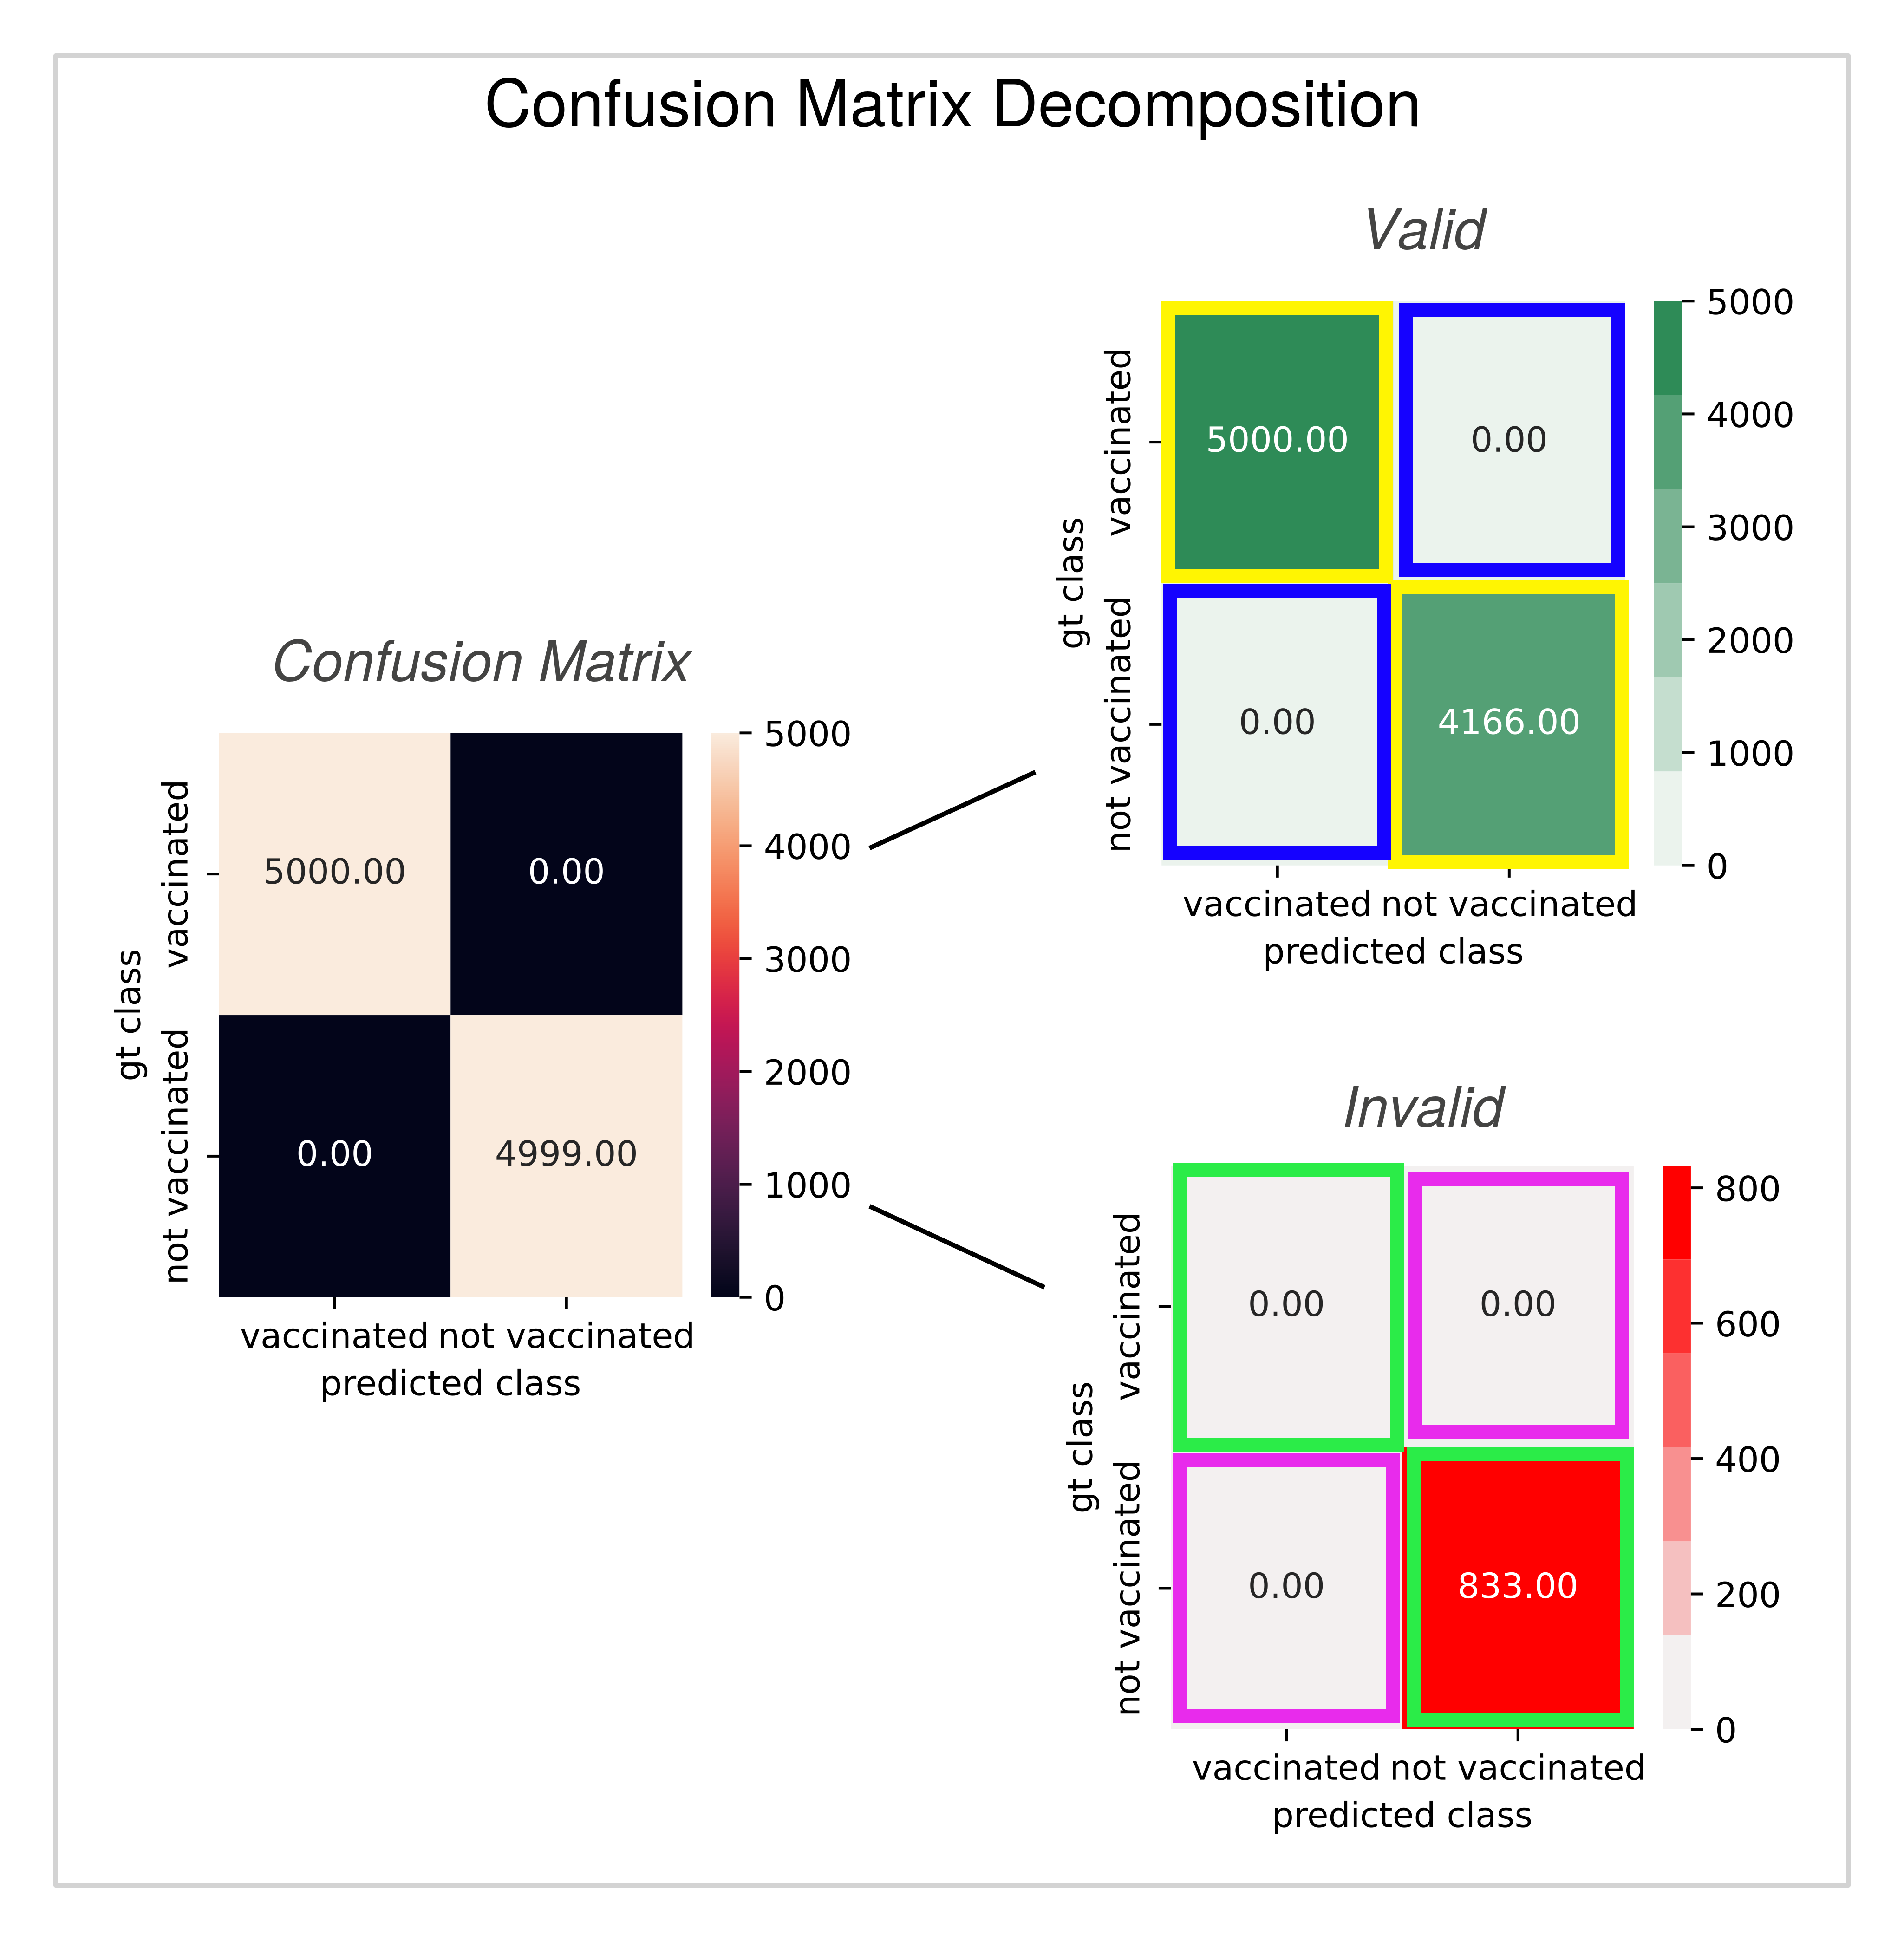
\includegraphics[scale=.08]{images/visualizations/confusion_matrix_decomposition_valid_invalid_marked.png}     
    \caption{Decomposing the Confusion Matrix into Its Valid and Invalid Components}
    \label{fig:confusion_matrix_decomposition_valid_invalid}
\end{figure}

Besides the decomposition of the confusion matrix, this approach could also be used for other kind of frequency distribution tables using a two-dimensional grouping function $\Gamma_{[1,2]}: G_1 \times G_2 \mapsto \mathcal{P}([1,...,N])$. In this case, the matrix on the left needs to use the entries of the frequency distribution that result when the validation results are summed per group $(g_1,g_2) \in G_1 \times G_2$.